\chapter{Future Work}\label{c:currWork}

This chapter provides a brief introduction over the problems that this dissertation aims to tackle, supported by a graphical dissertation schedule, in which the main development tasks are organized over time.

Following the \textit{Literature review} period where background concepts were duly studied and the pre-dissertation was written, it is expected that within the next first month security-related discussions will take place as major priority, due to its critical role on what this dissertation aims to tackle. Properties regarding security will be properly supported by ROS examples. Thus, it is intended to find concrete example that fails to address a specific security property, where the latter would be previously evaluated in a speculative manner. 

Afterwards, the already discussed schedule and respective assigned timings can proceed its predefined order. Here, ROS2 applications architectures will be formalized in Alloy, where the above's considerations about security and SROS2 configuration specification will be taken into account upon the modelling process. Then, it is expected to propose  a technique to specify and verify information-flow security properties on top of the proposed Alloy formalization.

Both \textit{Evaluation} and \textit{Implementation} periods will follow the latter's objectives. After concluding the \textit{Implementation}, the dissertation writing and review will proceed in order to present the full work on paper.

\begin{figure}[H]
    \centering
    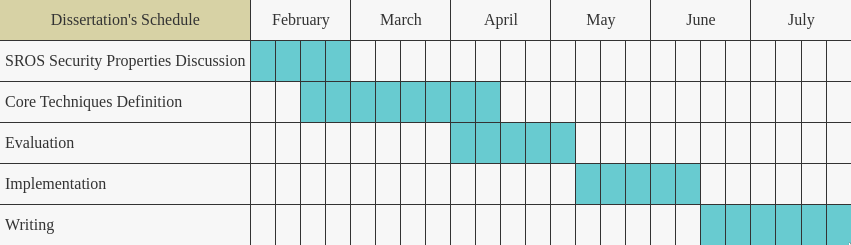
\includegraphics[width=\linewidth]{img/dissertation-schedule.png}
    \caption{Dissertation's schedule.}
    \label{fig:dissertation-schedule}
\end{figure}

The whole timetable is displayed above in the form of a table (Figure \ref{fig:dissertation-schedule}), with the times evenly split among the several periods. 
A more thorough schedule with related sub-tasks is shown below to completely contextualize the whole work that is planned to occur.

\begin{itemize}
\item SROS2-related Security Properties:
    \begin{itemize}
        \item Discussion and Overview.
    \end{itemize}

\item Core Techniques Definition:
    \begin{itemize}
        \item Formalization of the architecture of ROS2 applications in Alloy.
        \item Extend this formalization to cover the SROS2 security configuration.
        \item Propose a technique to specify and verify information-flow security properties on top of the proposed Alloy formalization.
    \end{itemize}

\item Evaluation:
    \begin{itemize}
        \item Selection of relevant case studies in the \textit{Autoware} platform.
        \item Identify and formalize relevant information-flow security properties for that case study.
        \item Evaluate the effectiveness of the proposed formalization and verification technique on the identified case studies and security properties.
    \end{itemize}

\item Implementation:
    \begin{itemize}
        \item Implement a prototype tool that can automatically infer an Alloy formalization of a ROS2 architecture and SROS2 security configuration.
    \end{itemize}

\item Writing:
    \begin{itemize}
        \item Finish dissertation writing.
        \item Dissertation review.
    \end{itemize}
\end{itemize}